\subsection{Student Grades}

\subsubsection{Statement}
Write a program in C that uses a two-dimensional array to store the numeric grade for
each student (n) in a multiple teacher’s class (m). The program assumes that the teacher has three
classes and a maximum of 30 students per class. Both the variable M and N should be user
defined.

\subsubsection{Code}
\inputminted[]{c}{../Code/student_grades.cpp}
\subsubsection{Output}
\begin{figure}[!htb]
  \centering
  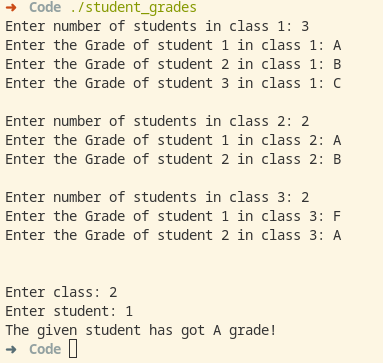
\includegraphics[width=4in]{Images/1.png}
  \label{Output-1}
  \caption{Output - 1}
\end{figure}

\pagebreak
\subsection{Average Age}

\subsubsection{Statement}
Write the program to input the value of age of employees in the company. You have to
calculate the average age of the employee in the company using pointer of array.

\subsubsection{Code}
\inputminted[]{c}{../Code/average_ages.cpp}
\pagebreak
\subsubsection{Output}
\begin{figure}[!htb]
  \centering
  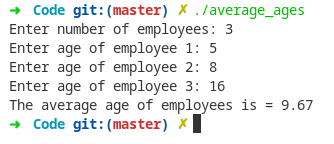
\includegraphics[width=4in]{Images/average.png}
  \label{Output-2}
  \caption{Output - 2}
\end{figure}


\pagebreak
\subsection{Length of string}

\subsubsection{Statement}
A user has given a random size string to input, you have to calculate the length of the
string using pointer. You cannot use predefined function strrev.

\subsubsection{Code}
\inputminted[]{c}{../Code/strlen.cpp}
\subsubsection{Output}
\begin{figure}[!htb]
  \centering
  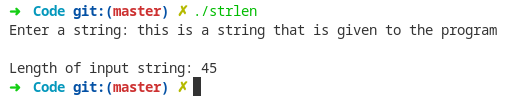
\includegraphics[width=4in]{Images/strlen.png}
  \label{Output-3}
  \caption{Output - 3}
\end{figure}

\pagebreak
\subsection{Start-Up Owner}

\subsubsection{Statement}
A start-up owner is interested to maintain the dataset of the newly recruited employees.

She is interested in storing the Emp\_Name (Str), Emp\_Age (int), Emp\_Degree (Str), Emp\_Exp
(Float), Emp\_add (Structure). Emp\_add needs one user defined data to store street no, city,
district and state for the employee address. You have to design a database where we can store all
the information for at least 20 employees.

\subsubsection{Code}
\inputminted[]{c}{../Code/employee.cpp}
\pagebreak
\subsubsection{Output}
\begin{figure}[!htb]
  \centering
  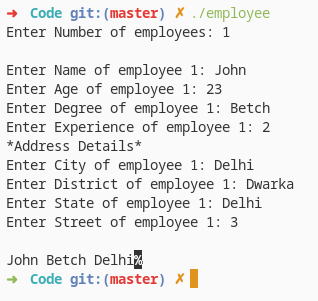
\includegraphics[width=4in]{Images/employee.png}
  \label{Output-4}
  \caption{Output - 4}
\end{figure}


\pagebreak
\subsection{Student Names}

\subsubsection{Statement}
Defined a two-dimensional matrix (char)[50][20] to store the student’s name in the class.
We are expecting to store the 50 students with different length name. Write a program to print all
the name with the help of pointers

\subsubsection{Code}
\inputminted[]{c}{../Code/students.cpp}
\subsubsection{Output}
\begin{figure}[!htb]
  \centering
  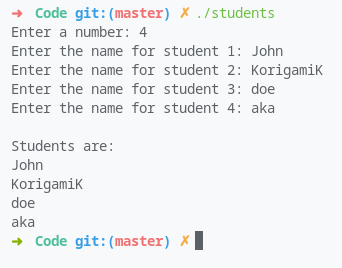
\includegraphics[width=4in]{Images/student_names.png}
  \label{Output-5}
  \caption{Output - 5}
\end{figure}

\pagebreak
\subsection{XOR Operation}

\subsubsection{Statement}
The outcome of a XOR operation is true if and only if one operand (but not both) is true. Write
a program in 'C' which returns the outcome of an Exclusive OR operation performed on its two
operands

\subsubsection{Code}
\inputminted[]{c}{../Code/xor.cpp}
\subsubsection{Output}
\begin{figure}[!htb]
  \centering
  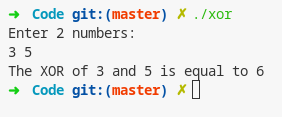
\includegraphics[width=3.5in]{Images/xor.png}
  \label{Output-6}
  \caption{Output - 6}
\end{figure}


\pagebreak
\subsection{Left and Right Shift}

\subsubsection{Statement}
Write a program in C to show that Right shift effectively divides a number by 2 and a left shift
effectively multiplies a number by 2

\subsubsection{Code}
\inputminted[]{c}{../Code/shifts.cpp}
\subsubsection{Output}
\begin{figure}[H]
  \centering
  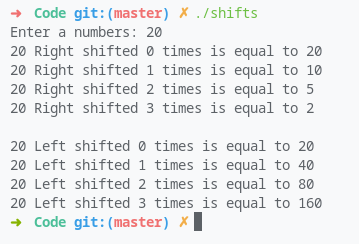
\includegraphics[width=4in]{Images/shifts.png}
  \label{Output-7}
  \caption{Output - 7}
\end{figure}


\pagebreak
\subsection{Magic Number}

\subsubsection{Statement}
Using the ? Operator, rewrite the magic number program discussed in the class

\subsubsection{Code}
\inputminted[]{c}{'../Code/magic_number.cpp'}
\subsubsection{Output}
\begin{figure}[!htb]
  \centering
  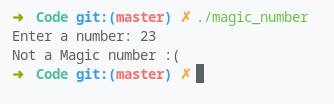
\includegraphics[width=4in]{Images/magic_number.png}
  \label{output-8}
  \caption{Output - 8}
\end{figure}


\pagebreak
\subsection{Quotient}
\subsubsection{Statement}
Using if else statement write a program in ‘C’ to read two integers from the user and display
the quotient. Your program should be able to detect divide by zero.
\subsubsection{Code}
\inputminted[]{c}{../Code/quotient.cpp}
\subsubsection{Output}
\begin{figure}[!htb]
  \centering
  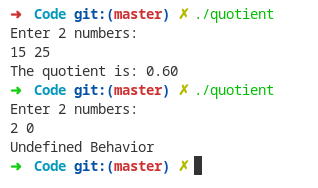
\includegraphics[width=4in]{Images/quotient.png}
  \label{Output-9}
  \caption{Output - 9}
\end{figure}


\pagebreak
\subsection{Text File}
\subsubsection{Statement}
Write a program in C that inputs lines of text until a blank line is entered. Then it redisplays
each line one character at a time
\subsubsection{Code}
\inputminted[]{c}{../Code/print_lines.cpp}
\subsubsection{Output}
\begin{figure}[!htb]
  \centering
  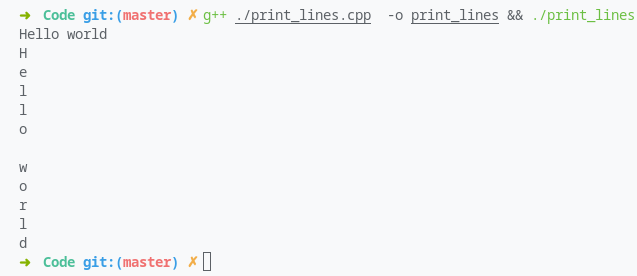
\includegraphics[width=5in]{Images/print_lines.png}
  \label{Output-10}
  \caption{Output - 10}
\end{figure}

\pagebreak
\subsection{Queue}
\subsubsection{Statement}
Write a program in C using pointers to implement insertion and deletion in a queue. A queue
is a data structure that follows a first in first out i.e. the element to go in first is the one to come
out first
\subsubsection{Code}
\inputminted[]{c}{../Code/q.cpp}
\pagebreak
\subsubsection{Output}
\begin{figure}[!htb]
  \centering
  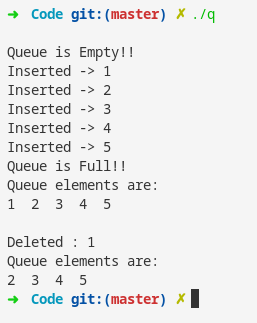
\includegraphics[width=3in]{Images/q.png}
  \label{Output-11}
  \caption{Output - 11}
\end{figure}


\pagebreak
\subsection{Temperature Conversion}
\subsubsection{Statement}
Write a program to print the corresponding celsius to Fahrenheit table. Modify the
temperature conversion program to print the table in reverse order, that is from 300 to 0
\subsubsection{Code}
\inputminted[]{c}{'../Code/temperature.cpp'}
\subsubsection{Output}
\begin{figure}[!htb]
  \centering
  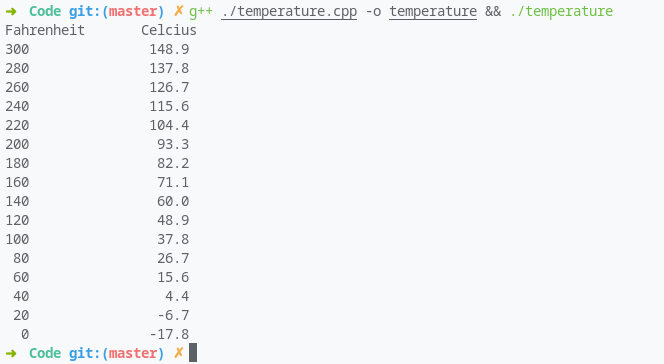
\includegraphics[width=6in]{Images/temperature.png}
  \label{Output-12}
  \caption{Output - 12}
\end{figure}


\pagebreak
\subsection{Text in File}
\subsubsection{Statement}
Write a program to count blanks, tabs and newlines
\subsubsection{Code}
\inputminted[]{c}{../Code/input_info.cpp}
\subsubsection{Output}
\begin{figure}[!htb]
  \centering
  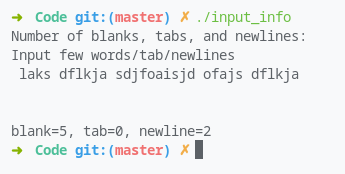
\includegraphics[width=4in]{Images/input_info.png}
  \label{Output-13}
  \caption{Output - 13}
\end{figure}


\pagebreak
\subsection{Frequencies}
\subsubsection{Statement}
Write a program to print the histogram of the frequencies of different characters of its input.
\subsubsection{Code}
\inputminted[]{c}{../Code/histogram.cpp}
\pagebreak
\subsubsection{Output}
Input Text
\begin{figure}[!htb]
  \centering
  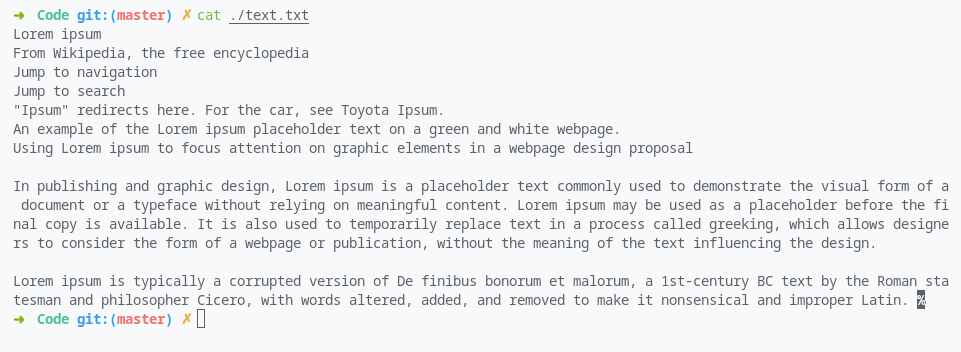
\includegraphics[width=6in]{Images/text.png}
  \label{Output-14-Text}
  \caption{Output - 14 - Text}
\end{figure}

Histogram
\pagebreak
\vspace*{-2.3cm}
\begin{figure}[H]
  \centering
  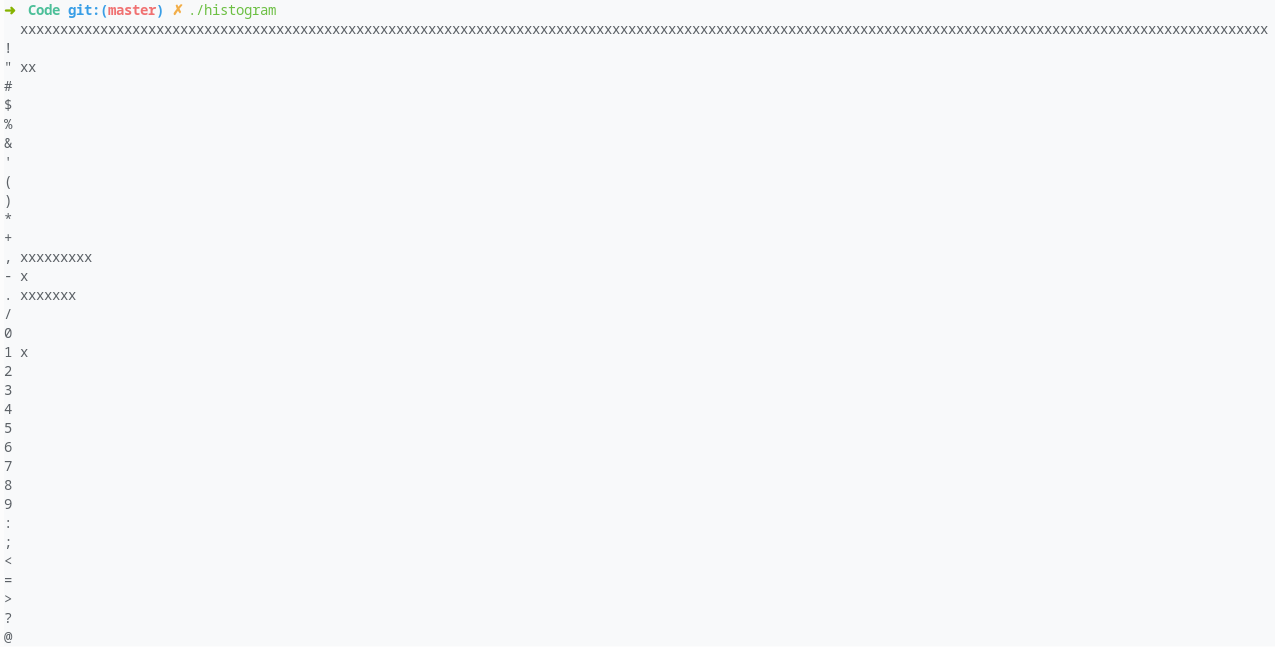
\includegraphics[width=6in]{Images/histogram1.png}
  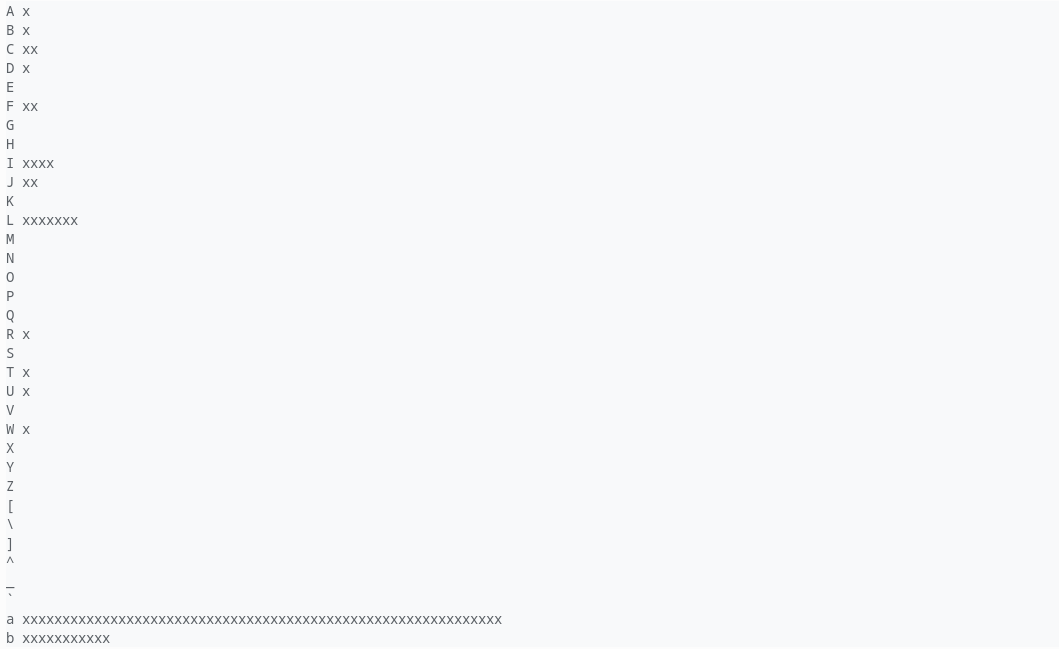
\includegraphics[width=6in]{Images/histogram2.png}
  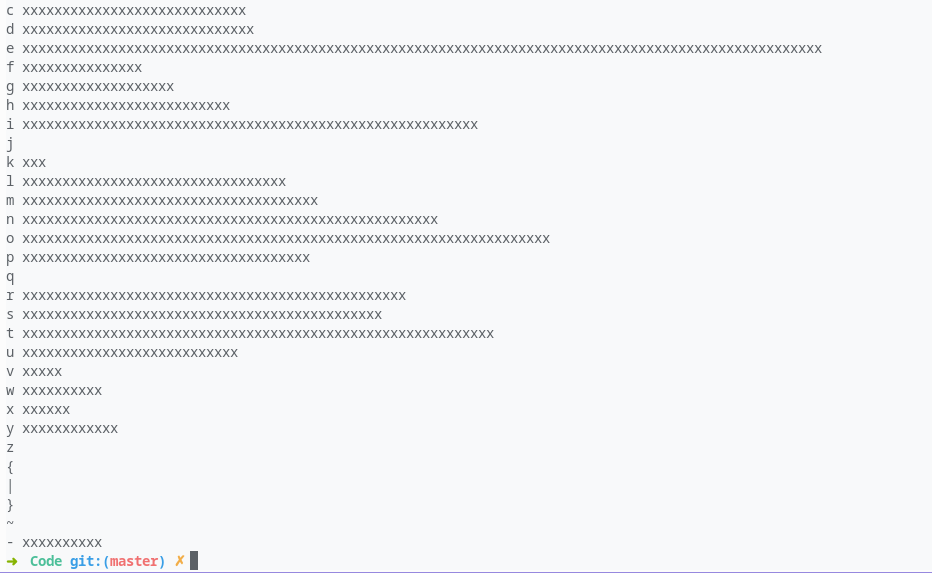
\includegraphics[width=6in]{Images/histogram3.png}
  \label{Output-14-Histogram}
  \caption{Output - 14 - Histogram}
\end{figure}
\pagebreak